% \subsection*{Design and Methods}

% Weak Scalability Design : Keep Pipeline of Ensembles to show barrier needed in S5 and S6
% Performance, generality with weak scaling (agnostic to kernel)
% Added functionality (do not speak about binding adaptivity to performance or generality)
% In use case: add in why TIES is challenging, and why adaptivity is challenging

% add in pseudo plots for weak, strong,

% For both free energy protocols ESMACS and TIES, each protocol instance
% represents a single EnTK pipeline. Both protocols requires a new pipeline to
% study each physical system. \jhanote{the above two sentences need to be
% clarified. not sure why they are in the experiments section.} Pipelines are
% executed concurrently.

For the TIES protocol, each pipeline consists of six stages. Each of the simulation
stages contains a task for every unique ($\lambda$, replica) combination.


%EnTK manages the
%queueing of the tasks in accordance with the order and concurrency mandated by
%stages and pipelines. \jhanote{.. need clean separation of implementation
%details from design of experiments}


In the non-adaptive workflow scenario, the first 11 $\lambda$ windows consist
of the following values: $L$ is a vector with
\begin{flalign}
L &= \{ x_i: x_i\in[0,1]\; and\; x_{i+1} = x_i + \delta \}, where\ \delta\ is\ 0.1.
%&$$L=\{ x_i: x_i\in[0,1]\; and\; x_{i+1} = x_i + \delta \}$$%, where $\delta$ is $0.1$.
\end{flalign}

  We append two additional values on both ends of $L$, completing 13 $\lambda$
windows. Each $\lambda$ window consists of five replicas. Therefore there are
a total of 65 tasks for every simulation stage. The production simulations
stage, $s4$ as described in figure~\ref{fig:pst} executes a 4 ns simulation duration. The analysis stages of
the protocol reduce the number of tasks. The first analysis task consists of
five tasks where each task performs an aggregate analysis over all $\lambda$
windows for each replica. The second analysis stage consists of one task that
aggregates the previous results and computes a single average across all
replicas.

%------------------------------------------------------------------------------

\subsubsection{Adaptive experiments}

The TIES workflow can benefit from an adaptive execution environment to improve
the efficiency and accuracy of the result. In \emph{adaptive experiments} we
implemented the adapative quadrature algorithm specifically customised for
biosimulations.

In the adaptive workflow, over the course of a protocol instance we alter
the number of $\lambda$ windows being simulated. The position of new $\lambda$
windows depends on the estimated error of the integral measured between
adjacent windows. Increasing the number of $\lambda$ windows in regions of
rapid change will increase the accuracy of the overall integral to a greater
degree than an
arbitrarily placed window. In order to adaptively add lambda windows, we need
access to the $dU/d\lambda$ values during runtime. Therefore, we break down the
single production simulation stage (S4) from the nonadaptive workflow into
multiple smaller stages, each running for 1 ns. Once each simulation is
complete within a stage a decision is made about whether more $\lambda$ windows
are required, and if so where they should be placed.

We start out the simulation with 5 replicas of \emph{3} equally spaced
$\lambda$ windows, and equilibrate them. Then repeatedly, we execute the
shorter production simultion followed by an analysis to determine where to
place new lambda windows. This is done until convergence, at which point all
concurrect simulation are terminated. Convergence is defined as the point in
the production-analysis loop when the desired error threshold has been
reached.  One of the key points in this algorithm is the decision to place more
lambda windows in certain domains. In adaptive quadrature, this is decided by
calculating an error estimate on the integral and deciding whether it is below
a certain threshold. Due to the stochastic nature of the biosimulations, it is
non-trivial to determine this error, and as a proof of concept we simplified
this decision to {\it a priori} calculated results. In future studies we plan
to replace this decision process with a more rigurous approach.

There is a constraint on the number of new lambda windows that can be added at
each iterations. To reduce overhead of inter-node communication, the
simulations have to run on an integer number of nodes. This means that the
number of new lambda windows (i.e. the number of simulations) \emph{has} to be
either doubled or left unchanged. In case of doubling the nodes per simulation can be automatically redistributed by halfing them. To achieve this the algorithm loops through the current lambda window pairs until this criterion is reached, forcefully adding more if needed.


% I don't think we need this equation here, it's too trivial.
% \begin{flalign}
% L &= \{ x_i: x_i\in[0,1]\; and\; x_{i+1} = x_i + \delta \}, where\ \delta\ is\ 0.5.
% %&$$L=\{ x_i: x_i\in[0,1]\; and\; x_{i+1} = x_i + \delta \}$$%, where $\delta$ is $0.1$.
% \end{flalign}

% For every $\lambda$ window we initialize with five replicas therefore yielding a
% total of 15 tasks. We run 15 tasks for stages $S1$ through $S4.1$. Between
% stages $S4.1$ and $S4.3$ the number of $\lambda$ windows doubles
% for every stage, which doubles the total number of tasks. The last production
% simulation stage, $S4.4$, runs for the remaining 2 ns durations.

HTBAC provides the functional capability to adaptively deterine the time at
which the $\lambda$ window are determined. However in this paper, we eschew a
discussion of this type of adaptivity, as the objective is to determine the
feasibility of adaptive execution and demonstrate the scientific merit of
implementing adaptive decision making. In order to provide "control" baseline
experiments, our experiments implement "adaptive change" not "when" i.e., we
introduce only a single degree of freedom relative to baseline "non-adaptive"
experiments.

\begin{figure}
  \centering
   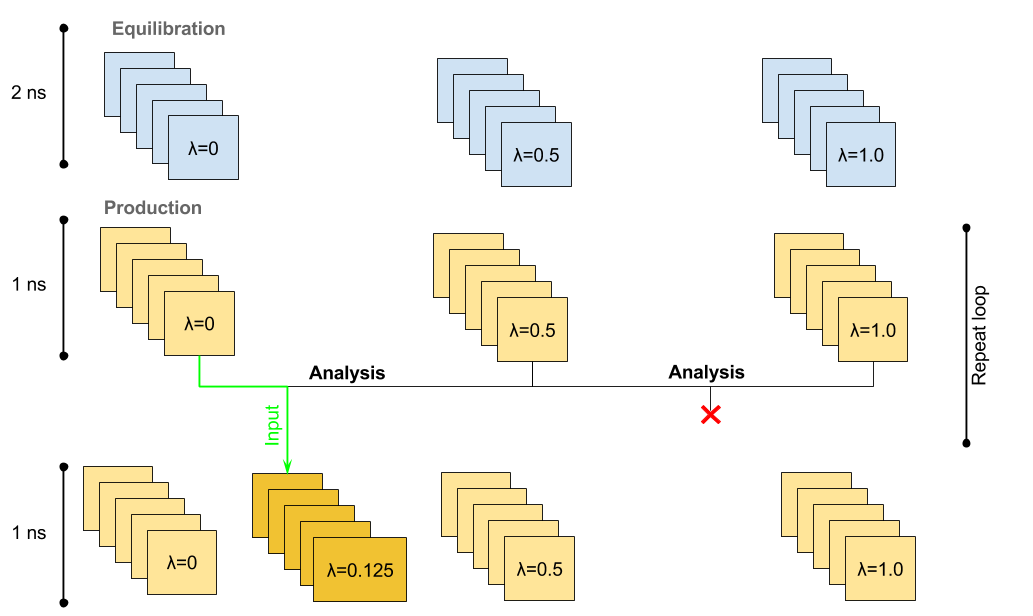
\includegraphics[width=\columnwidth]{figures/Adaptive_TIES_1.png}
  \caption{Illustrating the adaptive workflow. After the 3 inital lambda windows are equilibrated, the first production stage starts. This is followed by analysis at every lambda interval, to decide whether to add a new window in the middle. The production-analysis is repeated for 4 production steps in our implementeation, not shown here.}
\label{fig:adaptive_TIES}
\end{figure}


\subsection{Experiment Setup}\label{ssec:exp_design}

We perform weak (and strong) scalability experiments on NCSA Blue Waters--a
13.3. petaFLOPS Cray, with 32 Interlago cores/50 GB RAM per node, Cray Gemini,
Lustre shared file system. We perform our experiments from a virtual machine
hosted in Europe, as Blue Waters does not allow for executing applications
directly on the login node.

All experiments use HTBAC version 0.1, EnTK version 0.6 and RP version 0.47.
The MD engine used is NAMD-MPI for tasks pertaining to $S1$ - $S4$, while the
analysis stage, $S5$ use AmberTools. For both adaptive and nonadaptive
experiments, the minimization tasks of $S1$ are assigned 100(0) steps, while
the equilibration tasks in $S2$ and $S3$ are assigned 5000 steps. In the
nonadaptive experiments, the production simulation tasks in $S4$ are assigned
50000 steps. For the adaptive experiments, each substage of $S4$ i.e. $S4.1$ -
$S4.4$ is assigned X steps.

HTBAC submits a resource request to EnTK, to which EnTK uses RP to acquire
resources via a single pilot. Accordingly, we request the maximum number of
cores required by the workload as the number of cores in a pilot. We use
between 4160 and 33280 cores as indicated in figure~\ref{fig:weak_scaling}
because the NAMD executable used in all tasks from $S1$-$S4$ require at least
32 cores per task. From our own scalability performance measurements of NAMD
on Blue Waters, we observe the ideal cores per task to be 16, however Blue
Waters does not permit running multiple MPI applications on the same node,
hence each NAMD task requires a full node to maintain concurrency.

\begin{figure}
  \centering
   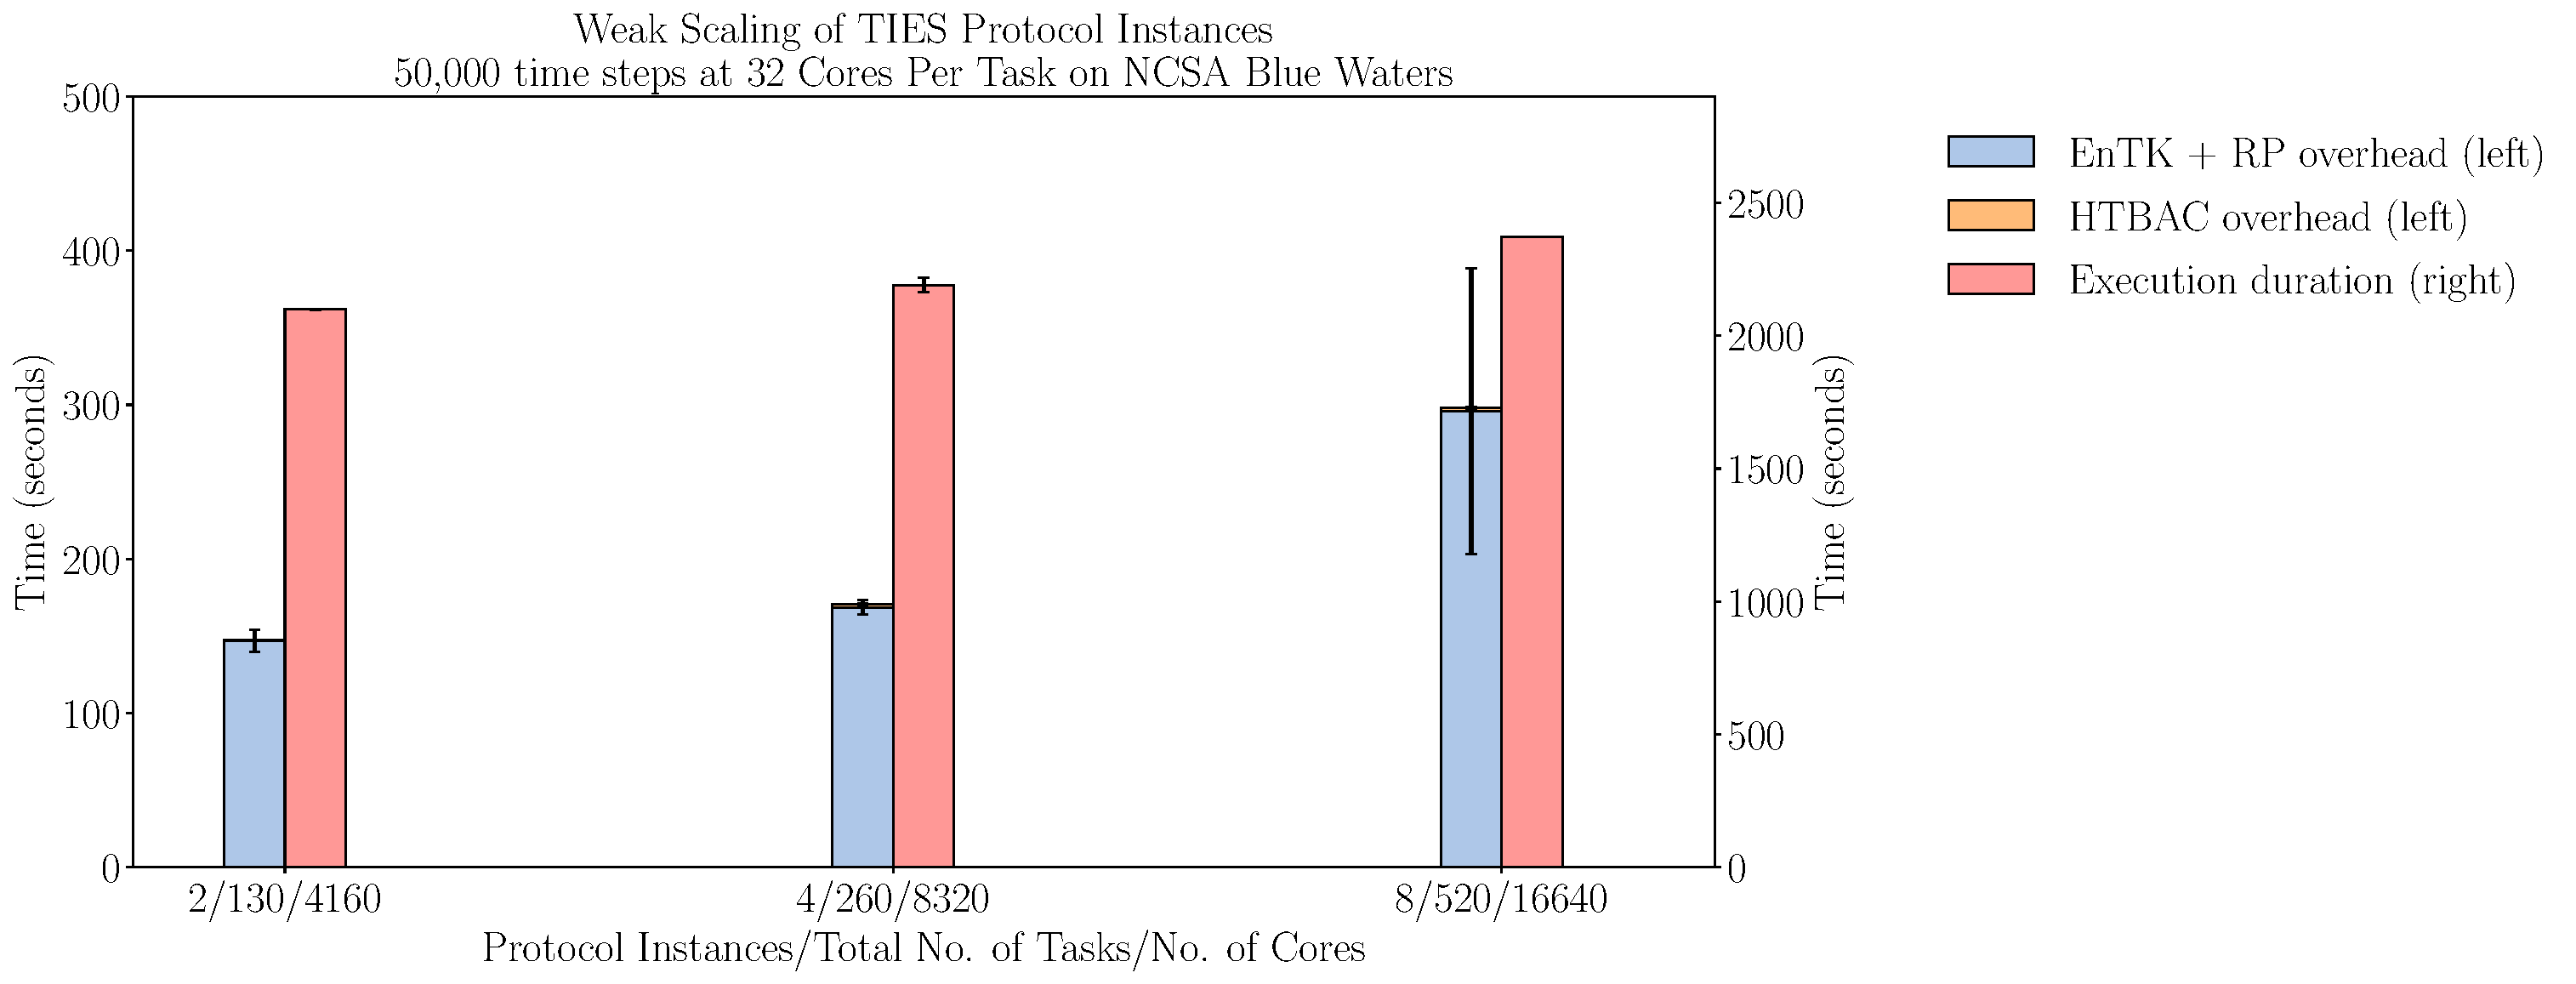
\includegraphics[width=\columnwidth]{./figures/weak_scaling_TIES_instances_50,000_timesteps.pdf}
  \caption{Weak scaling properties of HTBAC (right side). We investigate the
  weak scaling of HTBAC as the ratio of the number of protocol instances to
  resources is kept constant. (Left) Overheads of HTBAC, and runtime overhead (EnTK/RP) for
  experimental configurations investigating the weak scaling of TIES. We ran two trials for each protocol instance configuration.}
\label{fig:weak_scaling}
\end{figure}


<<<<<<< HEAD
HTBAC enables concurrent execution of multiple protocol instances.
With each new protocol instance generated for an
application, the HTBAC overhead grows to match the additional
requirement of generating and coordinating protocols. In order
to understand the contribution of the various events in HTBAC,
termed as HTBAC overhead, to the total time to run, we construct the following metrics:

\(Time-to-run = T(overhead\textsubscript{HTBAC} +
T(overhead\textsubscript{entk}) +
T(overhead\textsubscript{rp}) + T(execution)\). We define \(T(execution)\) as \(TTX = TTC - T_q\) where \(TTC\) is
time-to-completion and \(T_q\) is time spent queuing on the HPC machine.

\jhanote{We should discuss the above. It is difficult to follow..}

The remaining overheads, mainly EnTK and RP, depend on the number of tasks
that need to be translated in-memory from a Python object to a compute unit
(CU) description. As such, it is expected to grow proportionally to the number
of tasks. EnTK submits CU descriptions to a MongoDB used by RP, and the RP
pilot pulls these descriptions from the same database. This pull operation
occurs over a wide area networks, which introduces varying amounts of latency.

\(TTX\) measures the execution duration across all task, which includes pre-
executables, the main MD kernel execution, and post-executables.
=======

>>>>>>> e0352a35ec687a5fcb233c81c82ab6029aa7fbe4
